\documentclass{ximera}

%\addPrintStyle{..}

\begin{document}
	\author{Bart Lambregs}
	\xmtitle{Verticale worp}{}
    \xmsource\xmuitleg



%  Onze perceptie leert dat zwaardere lichamen sneller vallen dan lichtere. 
%  Een pluim en een steen komen in regel niet op hetzelfde moment op de grond terecht. 
%  Toch blijkt deze intuïtie niet te kloppen.
%  In het jaar 1586 stond een wetenschapper uit Brugge op de Nieuwe Kerk van Delft. 
%  \href{https://www.canonvanvlaanderen.be/events/simon-stevin/}{Simon Stevin} 
%  \footnote{Het woord wiskunde vindt zijn ethymologische stam in het Griekse \(\mu \alpha \theta \eta \mu \alpha \tau \iota \kappa \eta\), wat in ons alfabet overeenkomt met \mbox{\textit{math\=ematik\'e}}. Vandaag merk je deze invloed is het Franse \textit{mathématiques}, het Spaanse \textit{matemáticas}, het Turkse \textit{matematik}of het Zweedse \textit{matte}. Dat men in het Nederlandse taalgebied over \textit{wiskunde} spreekt, komt door Simon Stevin.}\footnotemark 
%  \footnotetext{Het woord fysica vindt zijn etymologische stam in het Griekse \(\phi \upsilon \sigma \iota \kappa \eta\), wat in ons alfabet overeenkomt met \mbox{\textit{physik\=\'e}}. Vandaag merk je deze invloed in het Franse \textit{physique}, het Spaanse \textit{física}, het Turkse \textit{fizik} of het Zweedse \textit{fysik}. Dat men in het Nederlandse taalgebied over de \textit{natuurkunde} spreekt, komt door Simon Stevin.}\footnotemark
%  \footnotetext{Voor \textit{de kunst van het scheiden} vervolledigt de lezer deze voetnoot zelf... (\mbox{\textit{kh\=em\=i\'a}, chimie, química, kimya, kemi}) }
%  liet vanop de kerktoren twee loden bollen met een verschillende massa vallen en stelde vast dat ze op hetzelfde moment de grond raakten. 
	


 Onze perceptie leert dat zwaardere lichamen sneller vallen dan lichtere. 
 Een pluim en een steen komen in regel niet op hetzelfde moment op de grond terecht. 
 Toch blijkt deze intuïtie niet te kloppen.
 In het jaar 1586 stond een wetenschapper uit Brugge op de Nieuwe Kerk van Delft. 
 \href{https://www.canonvanvlaanderen.be/events/simon-stevin/}{Simon Stevin}%
 \footnote{Het woord \textit{mathematica} vindt zijn etymologische stam in het Griekse 
 $\mu \alpha \theta \eta \mu \alpha \tau \iota \kappa \eta$, wat in ons alfabet overeenkomt met \textit{math\=ematik\'e}. Vandaag merk je deze invloed in het Franse \textit{mathématiques}, het Spaanse \textit{matemáticas}, het Turkse \textit{matematik} of het Zweedse \textit{matte}. Dat men in het Nederlandse taalgebied over \textit{wiskunde} spreekt, komt door Simon Stevin.\footnotemark}
 \footnotetext{Het Griekse $\phi \upsilon \sigma \iota \kappa \eta$, wat in ons alfabet overeenkomt met \textit{physik\'e}, is de ethomologische stam van het woord \textit{fysica}. Vandaag merk je deze invloed in het Franse \textit{physique}, het Spaanse \textit{física}, het Turkse \textit{fizik} of het Zweedse \textit{fysik}. Dat men in het Nederlandse taalgebied over de \textit{natuurkunde} spreekt, komt door Simon Stevin.\footnotemark}
 \footnotetext{Voor \textit{de kunst van het scheiden} vervolledigt de lezer deze voetnoot zelf... (\textit{kh\=em\=i\'a}, chimie, química, kimya, kemi)}
 
 liet vanop de kerktoren twee loden bollen met een verschillende massa vallen en stelde vast dat ze op hetzelfde moment de grond raakten.
 

 \begin{image}
 
 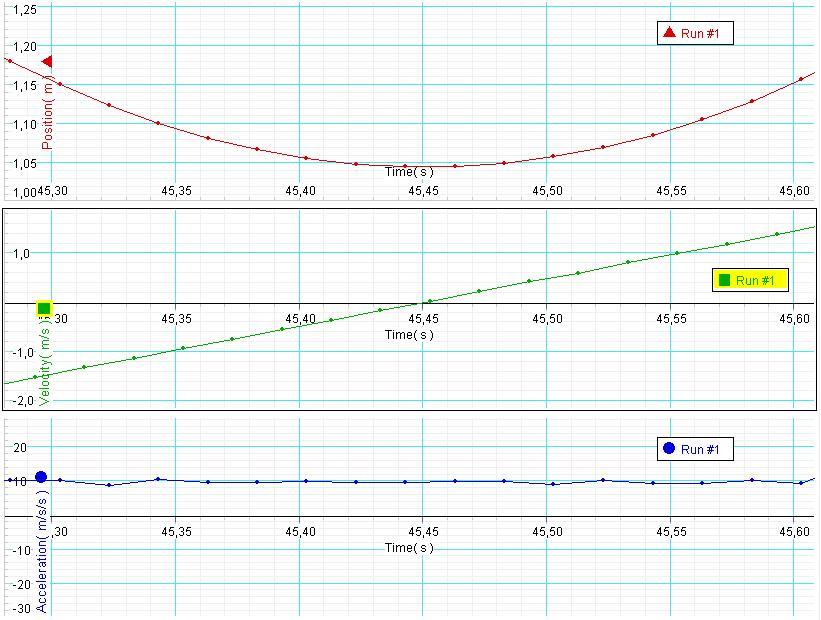
\includegraphics[width=0.85\textwidth]{valbeweging_pasco2}
 \end{image}
 \captionof{figure}{Experimenteel bekomen grafieken van een verticale worp waarbij de as naar beneden is georiënteerd.}

In vacuüm -- waar voorwerpen geen luchtweerstand ondervinden -- blijkt de massa geen rol te spelen bij de constante versnelling die de voorwerpen krijgen: alle voorwerpen vallen met dezelfde versnelling! 
Met lode bollen kon Simon Stevin het effect van de luchtweerstand uitschakelen. 
De theoretische verklaring voor dit experiment hoort thuis in de dynamica. 
In de kinematica wordt enkel de beweging beschreven. 
Omdat de valversnelling constant is, heb je hier simpelweg met een EVRB te maken.

Strikt genomen verschilt de valversnelling van plaats tot plaats op de aarde, maar voor het gemak nemen wij in vraagstukken de waarde
\[g=9,81\rm\,m/s^2.\]
Omdat de verticale worp een EVRB is, kunnen we de formules voor de plaatsfunctie en snelheidsfunctie gebruiken om een valbeweging te beschrijven. 
Voor de versnelling $a$ nemen we dan $a=g$ of $a=-g$ al naargelang de oriëntatie van de coördinaatsas.

\begin{quickquestion*}{}{}
Als je een tennisbal in de lucht gooit, op welk(e) moment(en) is de versnelling \(0\)? Op welk(e) moment(en) is de snelheid \(0\)? 
\end{quickquestion*}

\begin{quickquestion*}{}{}
Leg de fysische betekenis uit indien de zin van de snelheidsvector en versnellingsvector tegengesteld zijn. Wat indien ze dezelfde zin hebben?
\end{quickquestion*}
% volgend jaar hier de afbeelding van de basketbal invoegen 


\begin{exercise}
Simon Stevin laat van de boord van een schip een loden bol in het water vallen. De \mbox{boord} bevindt zich \SI{4}{\meter} boven het wateroppervlak. De loden bol zinkt vervolgens met de snelheid waarmee hij het water raakte. Er zijn \SI{6}{\second} tussen het loslaten van de bol en het raken van de bodem. 

\begin{image}
	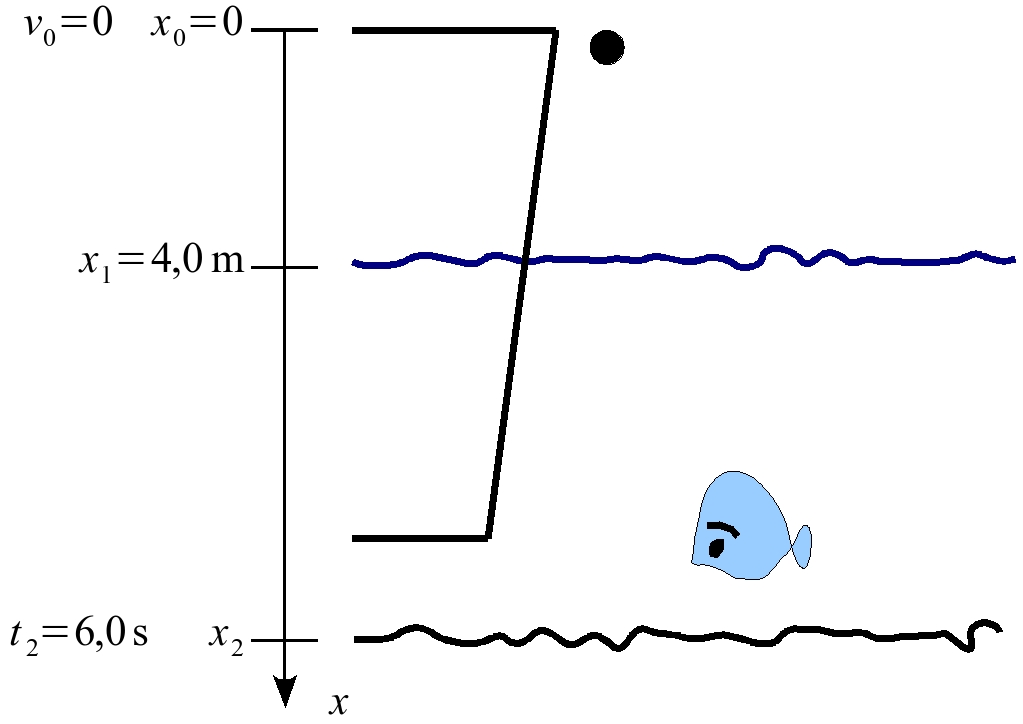
\includegraphics[width=0.4\textwidth]{boordschip}
\end{image}

\begin{question} Hoe diep is het water? 
\begin{oplossing}

	De beweging is opgebouwd uit twee verschillende soorten bewegingen. Het eerste stuk is een vrije val, wat een EVRB is. In het tweede stuk (onder water) is de snelheid constant en is er dus geen versnelling. In geen geval kunnen we dus de formules voor een EVRB op het geheel toepassen. Die zijn immers afgeleid voor een beweging waar de versnelling (altijd, gedurende de hele beweging) constant is. \\

	Omdat we weten hoe ver de bol moet vallen voordat hij het wateroppervlak bereikt, kunnen we zowel de tijd die de bol hiervoor nodig heeft als de snelheid waarmee de bol het wateroppervlak raakt, bepalen. We kiezen een as naar beneden zodat -- omdat de snelheid in deze richting toeneemt -- de versnelling positief is en gelijk aan de valversnelling $g$ (toch voor het eerste stuk). De beginsnelheid van de bol is nul omdat hij vanuit rust wordt losgelaten. Voor de tijd vinden we:
	
	\[
	x_1=\frac{1}{2}gt^2\quad\Rightarrow\quad t_1=\sqrt{\frac{2x_1}{g}}
	\]
	
	Met de tijd\footnote{We zouden de tijd met het gevonden formuletje kunnen uitrekenen en met het getalletje dat we vinden verder rekenen. Maar met het formuletje verder werken -- algebra\"isch of symbolisch -- is toch o zo veel knapper en van toepassing voor \'alle boten en niet enkel voor een boot waarvoor het dek zich $4,0$ meter boven het wateroppervlak bevindt. Bovendien is het ``echte'' fysica omdat je een ``model'' uitwerkt en niet een rekensommetje oplost...} kunnen we de snelheid op het wateroppervlak vinden.
	
	\[
	v_1=gt_1\nonumber=g\sqrt{\frac{2x_1}{g}}\nonumber=\sqrt{2gx_1}
	\]
	
	Onder water, in het tweede stuk, beweegt de kogel met deze snelheid gedurende de resterende tijd: $6,0$ seconden min de tijd $t_1$ (\ref{tijd_boordschip}) die de kogel nodig had om te vallen. De afstand die de bol onder water aflegt, vinden we met de eenvoudige formuletjes van een ERB\footnote{Opmerking, een ERB is een speciaal geval van een EVRB. Een ERB heeft als constante versnelling $a=0$.}. We substitueren ook vergelijkingen (\ref{tijd_boordschip}) en (\ref{snelheid_boordschip}).
	
	\[
	\begin{array}{rcl}
	\Delta x&=&\overline{v}\cdot\Delta t\\
	&\Downarrow&\\
	x_2-x_1&=&v_1(t_2-t_1)\\
	&=&\sqrt{2gx_1}(t_2-\sqrt{\frac{2x_1}{g}})\\
	&=&\sqrt{2gx_1}t_2-2x_1\\
	&=&45\rm\,m
	\end{array}
	\]

\end{oplossing}
\end{question}
\begin{question} Wat is de gemiddelde snelheid van de bol over het hele traject? \end{question}

\begin{oplossing}
% \textit{gegeven} $x_1=4,0\rm\,m$ \\%%%\newline$t_2=6,0\rm\,s$ \\
% \textit{gevraagd} $x_2-x_1$, $\overline{v}_{02}$ \\
% \textit{oplossing} 


De gemiddelde snelheid vinden we door de totale afgelegde weg te delen door de totale benodigde tijd. Andere formuletjes zoals $\overline{v}=\frac{v_1+v_2}{2}$ zijn niet van toepassing omdat het helemaal niet over \'e\'en EVRB gaat waar dit formuletje geldt omdat de snelheid mooi lineair toeneemt. Hier gebeurt dat enkel in het eerste stuk en worden de verschillende snelheden niet even lang aangehouden zodat ze een verschillend aandeel hebben in de totale benodigde tijd.

\[
\begin{array}{rcl}
\overline{v}_{02}=\frac{\Delta x}{\Delta t}=\frac{x_2}{t_2}&=&\frac{\sqrt{2gx_1}t_2-x_1}{t_2}\\
&=&\sqrt{2gx_1}-\frac{x_1}{t_2}\\
&=&8,2\rm\,m/s
\end{array}
\]

\end{oplossing}
\end{exercise}

\begin{xmuitweiding}[Een universiteitscollege over de leerstof van dit hoofdstuk.]
	\youtube{q9IWoQ199_o}
\end{xmuitweiding}

% \begin{expandable}{xmuitweiding}{Een universiteitscollege over de leerstof van dit hoofdstuk.}
% 	\youtube{q9IWoQ199_o}
% \end{expandable}

\end{document}